\documentclass[letterpaper, 10 pt, conference]{ieeeconf} 
\IEEEoverridecommandlockouts                             
\overrideIEEEmargins
\usepackage{amsmath,amssymb}
\usepackage{algorithm}
\usepackage{algpseudocode}
\usepackage{color}
\usepackage{graphicx}
\usepackage{multirow}
\usepackage{hyperref}

\title{
\LARGE \textbf{MADONNA}: A Framework for \textbf{M}easurements and \textbf{A}ssistance \newline in designing Low Power \textbf{D}eep \textbf{N}eural \textbf{N}etworks.
}

\author{Vinu Joseph and Chandrasekhar Nagarajan}

\begin{document}
\maketitle
\thispagestyle{empty}
\pagestyle{empty}

\begin{abstract}

The recent success of Deep Neural Networks (DNNs) in
classification tasks has sparked a trend of accelerating their
execution with specialized hardware. 
Since tuned designs easily give an order of magnitude improvement over
general-purpose hardware, many architects look beyond an MVP implementation.
This project presents Madonna v1.0, a direction towares automated
co-design approach across the numerical precision 
to optimize DNN hardware accelerators.
Compared to an 64-bit floating point accelerator
baseline, we show that 32-bit floating points accelerators, reduces energy by 1.5×;
Training time improved by 1.22x and a observable improvement in Inference as well;
Across three datasets, these power and energy measurements provide a collective average
of 0.5W reduction and 2x energy reduction over an accelerator baseline
without almost compromising DNN model accuracy. 
Madonna enables accurate, low power DNN accelerators , making it feasible to deploy
DNNs in power-constrained IoT and mobile devices.  

\end{abstract}


\section{INTRODUCTION}
Deep Neural Networks (DNNs) are Machine Learning (ML) methods that learn
complex function approximations from input/output examples.
These methods have gained popularity over the last 10 years, this gain
is attributed in NN literature to emirical achievenments on a wide range
of tasks that range from speech recognition, computer vision, and natural language processing. Apps that are based on DNNs can be found across
a broad range of computing spectrum, from large high power budget datacenters
down to a constrained power budget, battery-powered mobile and IoT deivices.
The recent success of DNNs in these problem domains are be attributed to 3 factors
\begin{enumerate}
  \item The availability of massive datasets
  \item Access to highly parallel computational resources such as GPU boards used in this paper.
  \item Improvements in the algorithms used to tune DNN's to data.
\end{enumerate}


The parameters (weights) of a DNN are fitted to data in a process called 
\textit{training}, which typically runs on a high performance CPU/GPU platform.
The training process depends on the charecteristics of the available data and
should ideally incorporate the latest advances in ML literature and practice,
those that are best suited to leverage the high flexibility of software.

During the \textit{prediction} phase, trained DNN models are used to infer
unknown outputs from input data that is new. \textit{training} is largely a 
one-time cost, inference  or prediction computations run repeatedly once
the DNN is deployed in the production environment.

\begin{figure}[h]
    \centering
    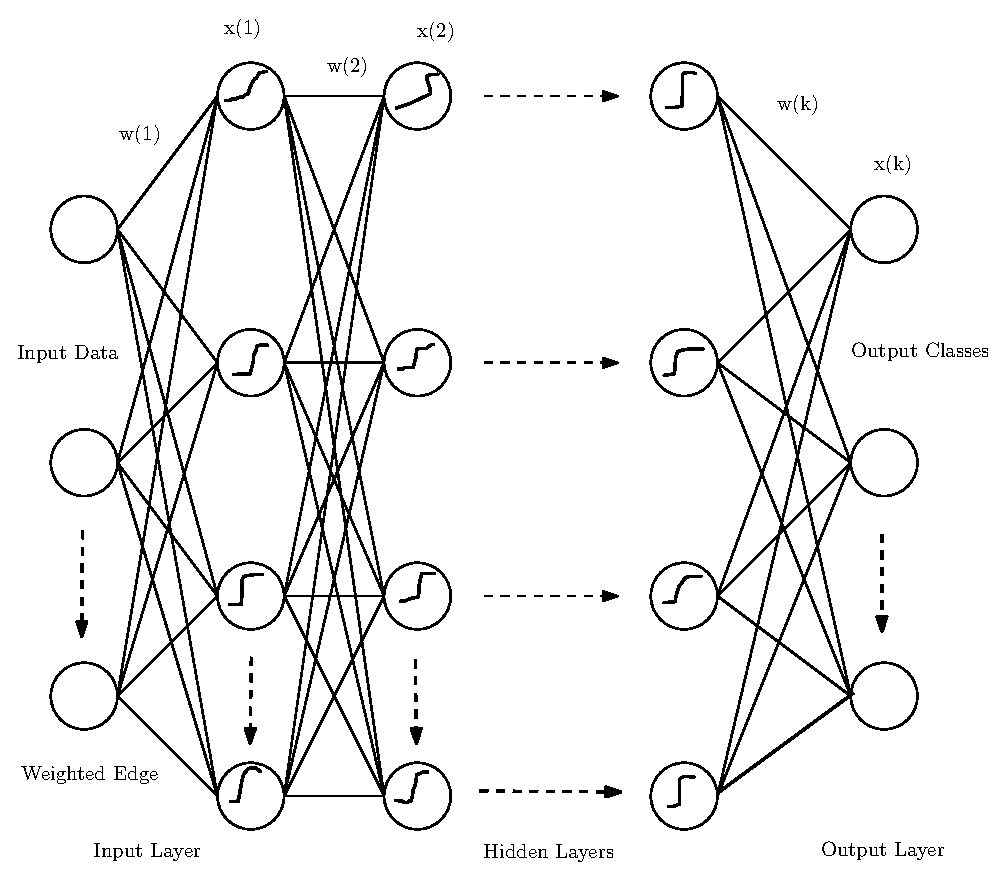
\includegraphics[width=85mm,scale=1.1]{nn}
    \caption{The operation of a DNN during the prediction phase as 
      a directed acyclic graph}
    \label{fig:nn}
\end{figure}
Therefore speeding up prediction and minimizing its power consumption is 
highly desirable, especially for apps that run on battery-powered devices with
strict power budgets and computational capabilities.

One of the solutions to this problem, which we studied in this course, is to
design and implement highly customized hardware accelerators for DNN predictions.
This project presents a holistic methodology , with an aim to assist the architect 
of DNN accelerators so that they can achieve minimum power while maintaining high prediction accuracy

MNIST is a widely studied dataset used by the ML community to demostrate state-of-the-art advances in DNN techniques. Figure \ref{fig:lenet_ds} shows the DNN used in this paper for this data set. As we studied in class there are 2 groups or community that is looking into improving DNN's. 

\begin{enumerate}
  \item ML community, focuses on minimizing prediction error and favours
        the computational power of GPU's over CPU's.
  \item HW commuity, focuses on reducing power consumption and silicon area, 
        moslty at the expense of non-negligible reductions in prediction accuracy.
\end{enumerate}

There is a divergence in the trends observed in the research outcomes of both
these teams, the Minerva tool we studied in class, revealed a notable gap
for implementations that achieve competitive prediction accuracy with power budgets 
within the grasp of mobile and IoT platforms.
In this project, we present Madonna, a framework to perform energy measurements
as the architect makes design decisions, this is motivated by the fact that 
embedded apps are running with strict power budget and to measure early will provide confidence to the designer that he/she is not making any high power design choices, (explained more in PROPOSAL)
Madonna has 4 steps, Launching tuned DNN on the embedded board, Initializing energy measurement setup, Postprocessing to visualize the running time , power and energy profile of the execution and Taking appropriate correcting action to meet the power, runtime budgets for the learning problem.
The 3 benchmark we simulated show that there considerable reduction in runtime, power and energy using our framework.


\section{BACKGROUND}

\subsection{Neural Nets}

Neural networks are a biologically inspired machine learning method
for a learning complex functions which apply mulpitle nonlinear
transformations to an input vector to obtain a corresponding output
vector.

\subsection{Deep Neural Nets}

Deep Neural networks (DNNs) are defined as networks with one or more
hidden layers.
The nonlinear tranformations are performed by consecutive layers
of fully connected artificial neurons.
The first layer is called the input layer, and it has a neuron
for each component in the input vector.
The last layer is called the output layer and contains one neuron
for each component in the output vector.
Between input and outout layers, there are additional layers
of hidden neurons.
The strength of the connection between neurons is determined
by a collection of weights whose values are tuned to minimize
the prediction error of the network on some training data.
Figure(\ref{fig:nn}) shows a DNN, represented as a weighted 
directed acyclic graph.  There are biological metaphors for 
all these, the are called synapses for edges and neurons for nodes.


\subsection{Training a DNN}

A neural network is trained by iteratively adjusting weights to minimize
 a loss function over labelled data.
Training is often performed using stochastic gradient descent (SGD), and 
the loss function is usually a combination of the prediction error and 
regularization terms. This process requires hyperparameter values related to
the network topology, for example the number of layers and neurons per layer
and the configuraion of the SGD procedure, for example the regularization
parameters. These hyperparameter values are often tuned by selecting, 
amoung a grid of candidates, values that minimize the prediction error
of the corresponding trained DNN. This can then be used to make predictions
on new inputs for which the corresponding outputs are not available.

\begin{algorithm}
\caption{Training a Deep Neural Network}
\begin{algorithmic}[1]
\Procedure{train}{}
\State {Initialize all weights $w_{ij}^{(l)}$ at \color{green} random}
\For {$t=0,1,2, \cdots ,do$}
  \State {Pick $n \in \{1,2,\cdots,N\}$ }
  \State { \color{blue} Forward: Compute all $x_j^{(l)}$}
  \State { \color{red} Backward: Compute all $\delta_j^{(l)}$}
  \State {Update the weigths: $w_{ij}^{(l)} \gets w_{ij}^{(l)} - \eta x^{(l-1)}_{i} \delta_{j}^{(l)}$  }
  \State {Iterate to the next step until it is time to stop}
\EndFor
 \State {Return the final weights $w_{ij}^{(l)}$}
\EndProcedure
\end{algorithmic}
\end{algorithm}


\subsection{Predictions using a DNN}

Each neuron output is obtained by computing a linear combination of the outputs
of the neurons in the previous layer and then applying a nonlinear function, 
where the first layer is fed by the input vector.
Equation(\ref{eq:infer}) summarizes this section, each $w_{ij}^{(l)} \in R$
represents the connection strength between the $i^{th}$ neuron in layer $(l-1)$
and $j^{th}$ neuron in the layer $(l)$. The nonlinear function $\theta$ allows
DNN's to become universal approximators. While many different non linear functions
have been proposed, recent research favors the rectifier because of its simplicity
and superior empirical performance.


\begin{align}
  w_{ij}^{(l)} &=
  \begin{cases}
    1 \le l \le L \text{  layers  } \\
    0 \le i \le d^{(l-1)} \text{ inputs  } \\
    1 \le j \le d^{(l)} \text{ outputs  }
  \end{cases} \\
  x_{j}^{(l)} &= \theta(s_{j}^{(l)}) = \theta\Bigg( \sum_{i=0}^{d^{(l-1)}}
                        w_{ij}^{(l)} x_{i}^{(l-1)}  \Bigg)    \\        
 \theta(s)  &= tanh(s) = \frac{e^{s} - e^{-s}}{e^s + e^{-s}} 
  \label{eq:infer}
\end{align}

\begin{align}
  { \text{ Apply } } \bf{x} \text{ to } x_{1}^{(0)}, &\cdots, x_{d^{(0)}}^{(0)}  \rightarrow \rightarrow x_{1}^{(L)} &= h(x) \\
\end{align}



          \begin{figure}[h]
              \centering
              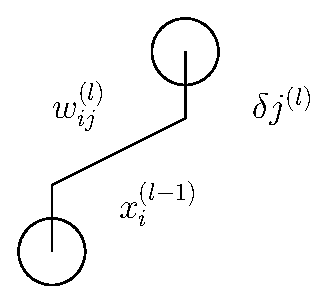
\includegraphics[width=50mm,scale=0.3]{train}
              \caption{Backpropagation used to train NN}
              \label{q1}
          \end{figure}


          \begin{figure}[h]
              \centering
              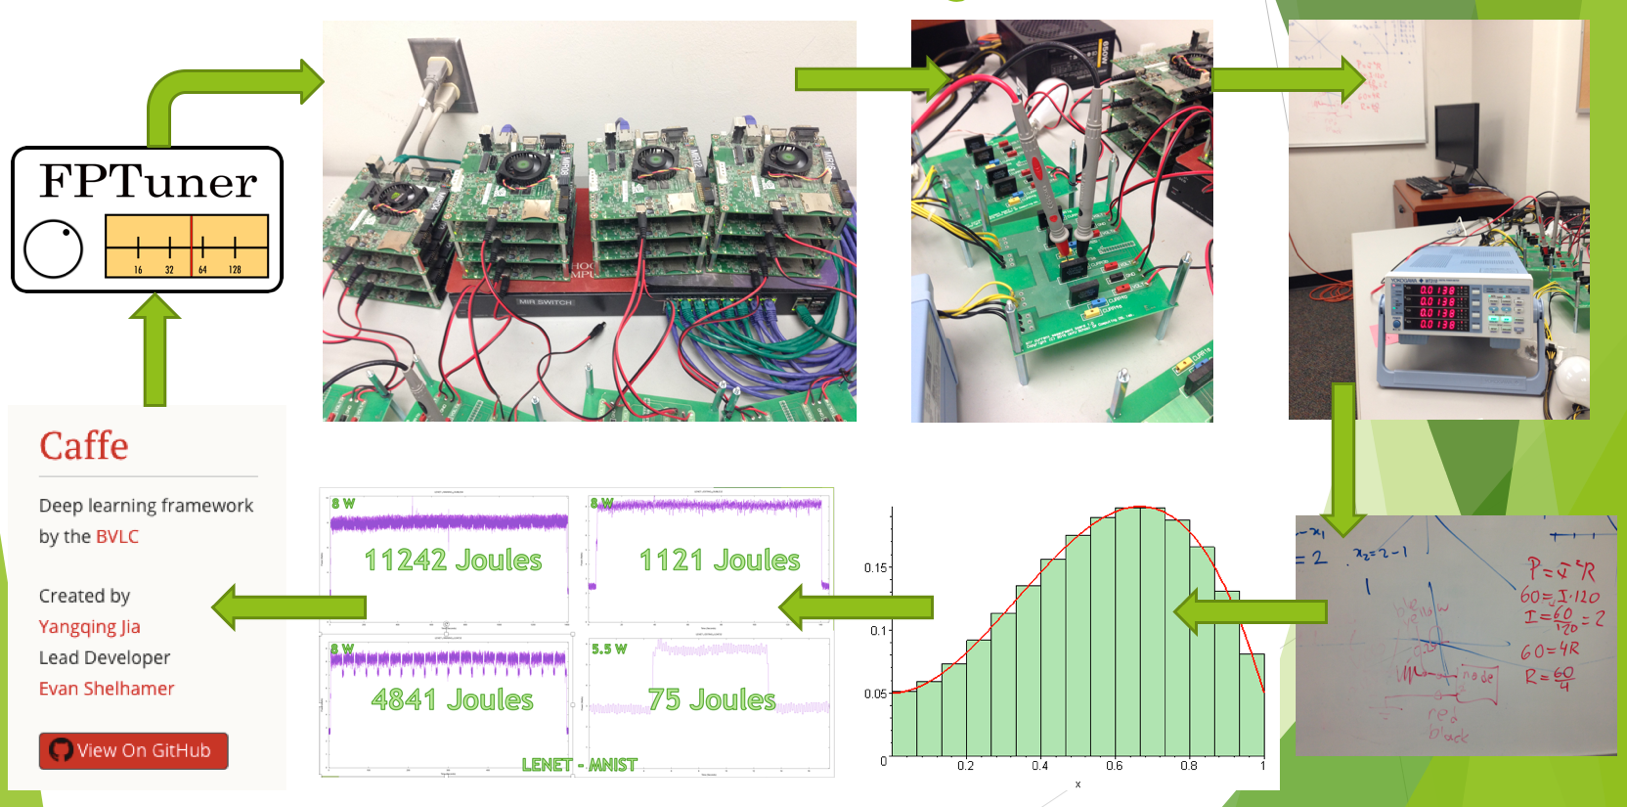
\includegraphics[width=85mm,scale=1]{wf}
              \caption{Workflow of Madonna, training LeNet on MNIST dataset}
              \label{q1}
          \end{figure}



\section{PROPOSAL}
         
Neural net architects who work on applications that are compute-intensive, especially on projects like Drones, Autonomous robotic systems, Mobile medical imaging, and Intelligent Video Analytics (IVA) are given strict power and running time budgets. They already have several design parameters to search over, for example which method to use to initialize weights, which activation function to use in which layer, which cost function to use, how to set the paramters like $\eta$, epochs mini-batch, $\lambda$ , how to expand the training data, how to go about regularization choices L1/L2 vs Dropout. 
One top of these, the fact that they need to tune for power, and numerical precision is very exausting, and the presence of tool in this area for assistance in making optimal choices and performing real energy measurements will be very useful. This is motivated by one of the lectures, we saw in class where we studied about Tools to explore accelerators, like Minerva tool to explore the design space, prune/quantize, lower voltages.
Madonna is a proposal in this direction, a tool to explore numerical precision part of the design space and perform measurements as one designs the network.

\begin{figure}[h]
  \centering
  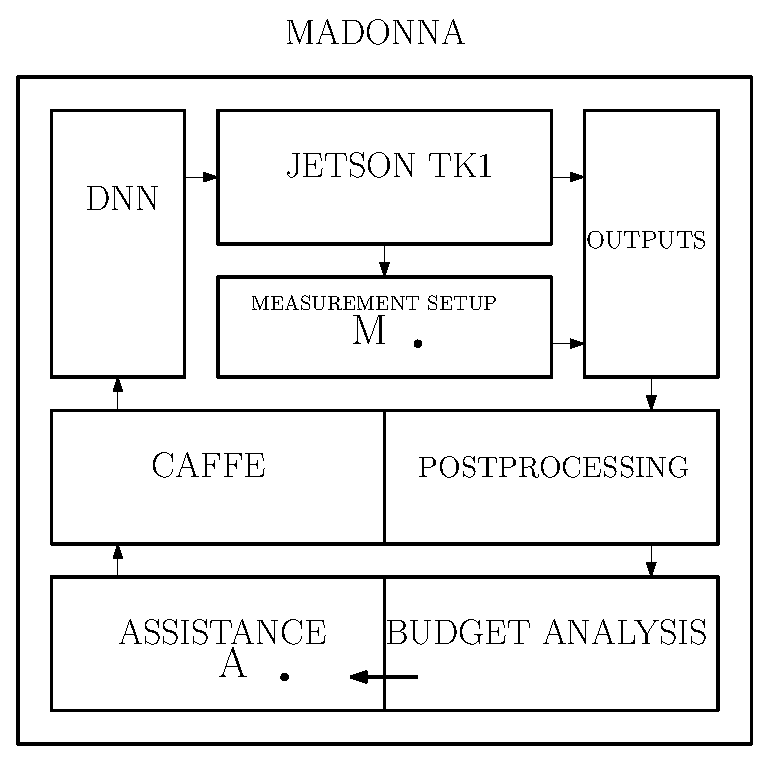
\includegraphics[width=70mm,scale=1]{frame}
  \caption{Block Diagram of our validated Framework}
  \label{fig:frame}
\end{figure}


          \begin{figure}[h]
              \centering
              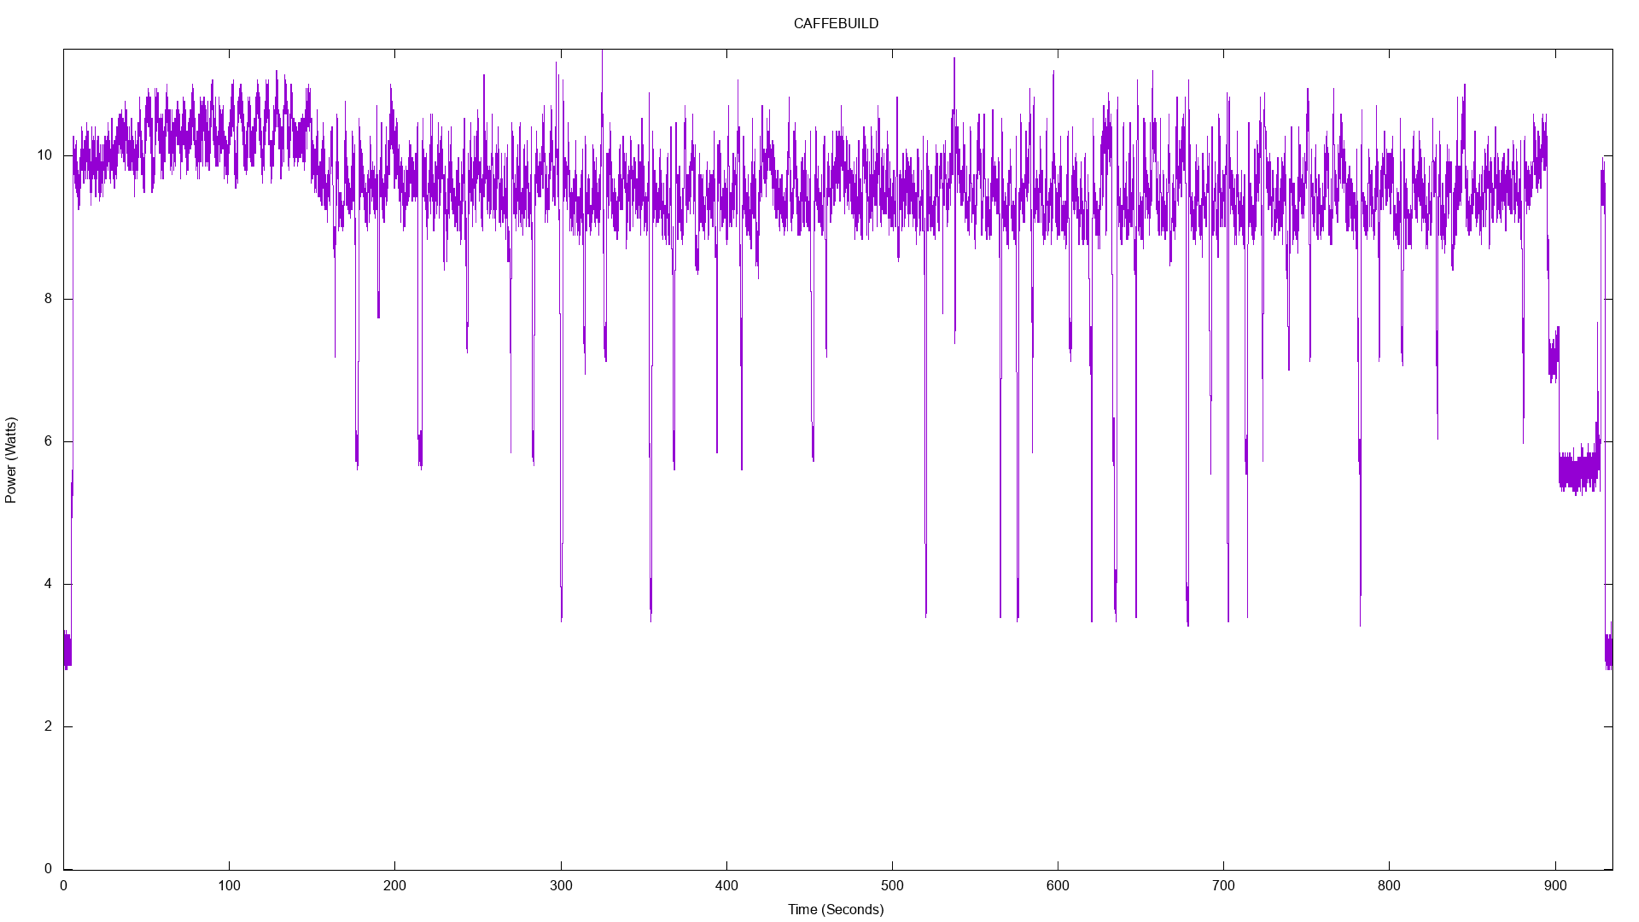
\includegraphics[width=85mm,scale=1]{caffe_make}
              \caption{Power profile while building The deep learning 
               framework Caffe, on Jetson TK1}
              \label{caffe_make}
          \end{figure}


\section{EXPERIMENTAL METHODOLOGY}

\subsection{Circuit Level}
\begin{itemize}
  \item The nodes are Nvidia Jetson TK-1 boards \url{http://elinux.org/Jetson_TK1}
  \item The measurement hardware is a Yokogawa  wt310 \url{http://tmi.yokogawa.com/us/products/digital-power-analyzers/digital-power-analyzers/digital-power-meter-wt300e/}
  \end{itemize}

\subsection{Topology, Network Level}

\begin{itemize}

  \item From a network prespective:

The head/gateway node is \verb|mir.cs.utah.edu| (mir) and users can acess it extrnally. 

\item mir is then connected to the switch on the table. This switch is then connected to the nvidia jetson tk-1 boards (mir01, mir02,.... mir16). To connect to them you must first ssh into mir then ssh into the desired node.

\item The power measurement computer, \verb|mirpwr.cs.utah.edu| (mirpwr), is only connected to the University of Utah nework.

\end{itemize}

\subsection{Electrical perspective}

\begin{itemize}
  \item Components that are directly connected to wall power with no measurement capabilities are mir, mirpwr, the switch, and the yokogawa.

  \item The two ATX power supplies are connected to the measurement PCB's, two PCSB's for each power supply. 
  \item Each measurement PCB has 4 shunt resistors on them and they power 4 mir nodes. 
  \item 8 nodes are being powered by each ATX power supply. The circuit for each measurement loop is simple, 
        there is a 12V supply ran through the dropper resistor, then the mir node, to ground.

\end{itemize}
\subsection{Framework}

Figure(\ref{fig:frame}) shows the block diagram of the MADONNA framework, the Assistance
block was studied but is not part of this version 1.0.

\subsection{Software}

\begin{itemize}
  \item Frontend   : The frontend for MADOANN 1.0 is is python, they essentially consisty of the 
  \item Backend    : Energy measurerement, trigger-measure-save steps are implemented in C++, and abstracted to the user via API's
  \item Validation : There are simple unit tests for each block (\ref{fig:frame})
  \item Debugging  : There is minimal debugging support now, and Hangs and Haults are attributed to fixed, known documented reasons.
  \item Download   : MADONNA 1.0 is Available for Download at GitHub \url{https://github.com/vinutah/madonna}

  \end{itemize}

  \subsection{Data Sets Evaluated}

          \begin{figure}[h]
              \centering
              \includegraphics[width=70mm,scale=1]{lenet_ds}
              \caption{LeNet on MNIST Data Set}
              \label{fig:lenet_ds}
          \end{figure}
          \begin{figure}[h]
              \centering
              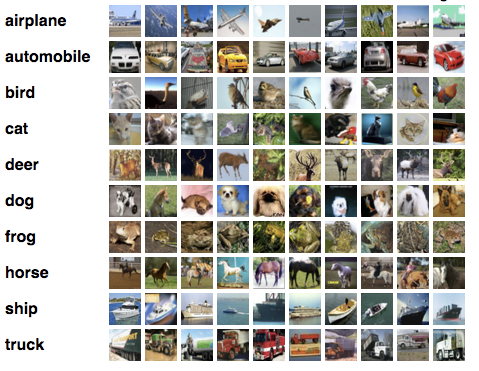
\includegraphics[width=70mm,scale=1]{cifar10_ds}
              \caption{CudaConvNet on CIFAR-10 Data Set}
              \label{cifar10_ds}
          \end{figure}
          \begin{figure}[h]
              \centering
              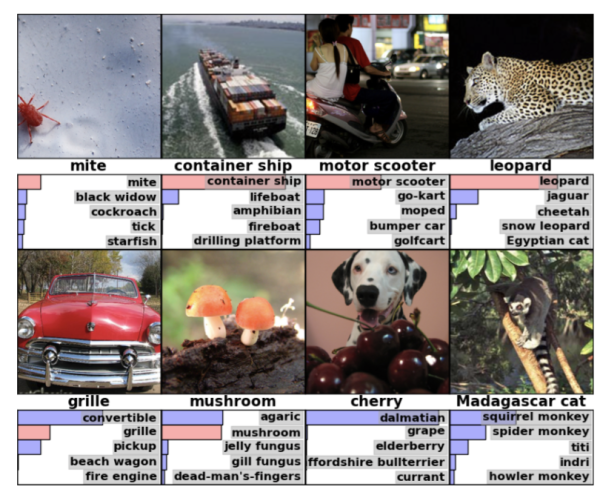
\includegraphics[width=70mm,scale=1]{imagenet_ds}
              \caption{CaffeReferenceNN on ImageNet Data Set}
              \label{imagenet_ds}
          \end{figure}


\section{RESULTS}


\begin{table}[ht]
  \centering
  \caption{IEEE-754 32-bit Double Precision Floating Point Represenetations}
  \label{my-label}
  \begin{tabular}{|c|c|c|c|c|c|}
    \hline
    \multirow{3}{*}{DATA SET} & \multicolumn{5}{c|}{SINGLE}                                                     \\ \cline{2-6} 
                              & \multicolumn{2}{c|}{TRAINING}                    & \multicolumn{3}{c|}{TESTING} \\ \cline{2-6} 
                              & POWER                  & ENERGY                  & POWER  & ENERGY  & ACC  \\ \hline
    MNIST                     & 7.5 W                  & 4492 J                  & 6.5W   & 35 J    & 97.5\%    \\ \hline
    CIFAR-10                     & 9.5 W                  & 11662 J                 & 10W    & 62 J    & 73.3\%    \\ \hline
    IMAGENET                  & \multicolumn{2}{c|}{Caffe Model Zoo}             & 13 J   & 722 J   & --        \\ \hline
  \end{tabular}
\end{table}

\begin{table}[ht]
  \centering
  \caption{IEEE-754 64-bit Double Precision Floating Point Represenetations}
  \label{my-label}
  \begin{tabular}{|c|c|c|c|c|c|}
    \hline
    \multirow{3}{*}{DATA SET} & \multicolumn{5}{c|}{DOUBLE}                                                     \\ \cline{2-6} 
                              & \multicolumn{2}{c|}{TRAINING}                    & \multicolumn{3}{c|}{TESTING} \\ \cline{2-6} 
                              & POWER                  & ENERGY                  & POWER  & ENERGY  & ACC  \\ \hline
    MNIST                     & 8 W                    & 10828 J                 & 8.0 W  & 50 J    & 98.8\%    \\ \hline
    CIFAR-10                     & 10 W                   & 31211 J                 & 10.5W  & 62 J    & 73.3\%    \\ \hline
    IMAGENET                  & \multicolumn{2}{c|}{Caffe Model Zoo}             & 13 J   & 722 J   & --        \\ \hline
  \end{tabular}
\end{table}

          \begin{figure}[h]
              \centering
              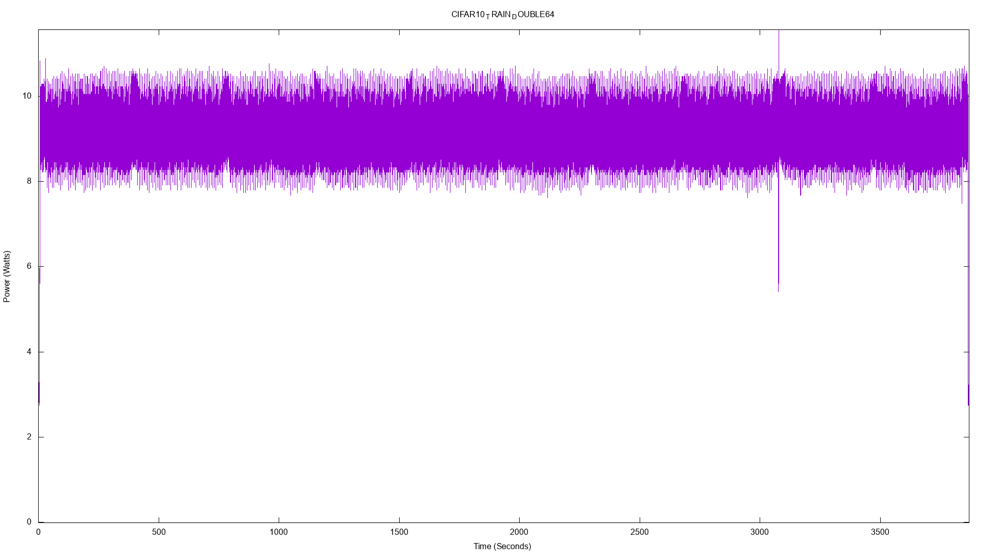
\includegraphics[width=85mm,scale=1]{cifar10_train_double.png}
              \caption{Training Cuda-Convnet on CIFAR-10 dataset, in double precision}
              \label{cifar10_train_double}
          \end{figure}

          \begin{figure}[h]
              \centering
              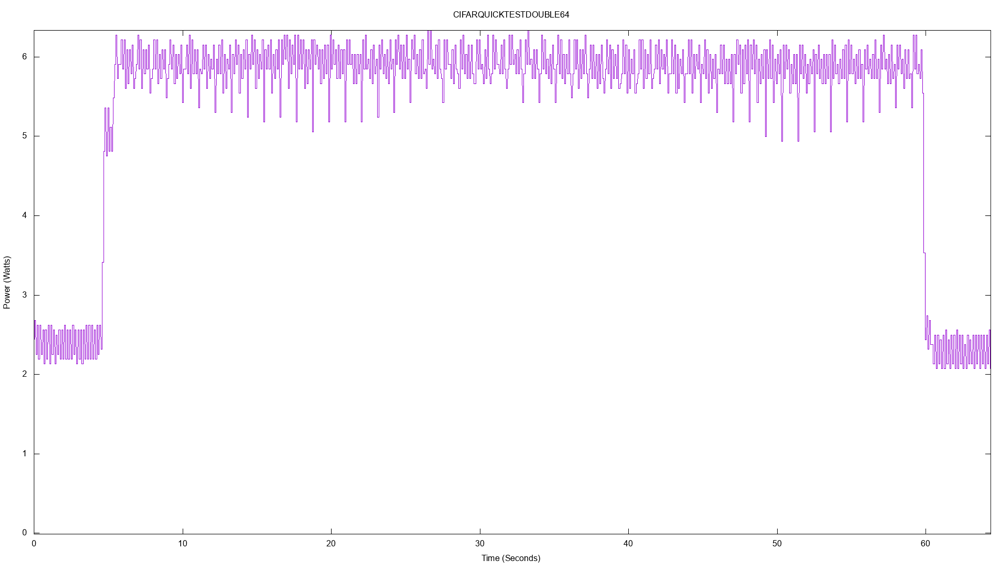
\includegraphics[width=85mm,scale=1]{cifar10_test_double.png}
              \caption{Testing Cuda-Convnet on CIFAR-10 dataset, in double precision}
              \label{cifar10_test_double}
          \end{figure}

          \begin{figure}[h]
              \centering
              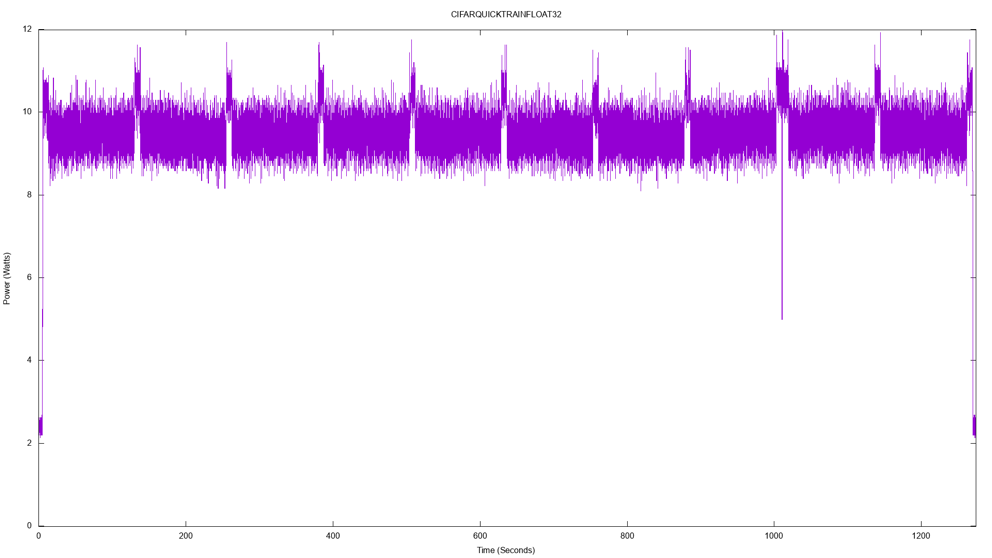
\includegraphics[width=85mm,scale=1]{cifar10_train_single.png}
              \caption{Testing Cuda-Convnet on CIFAR-10 dataset, in single precision}
              \label{cifar10_train_single}
          \end{figure}
          
          \begin{figure}[h]
              \centering
              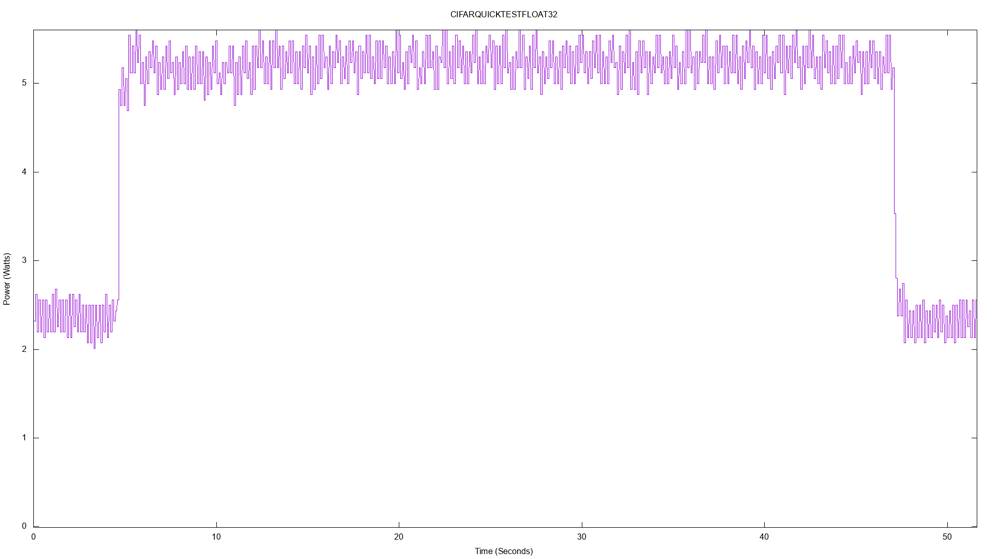
\includegraphics[width=85mm,scale=1]{cifar10_test_single.png}
              \caption{Testing Cuda-Convnet on CIFAR-10 dataset, in single precision}
              \label{cifar10_test_single}
          \end{figure}

          \begin{figure}[h]
              \centering
              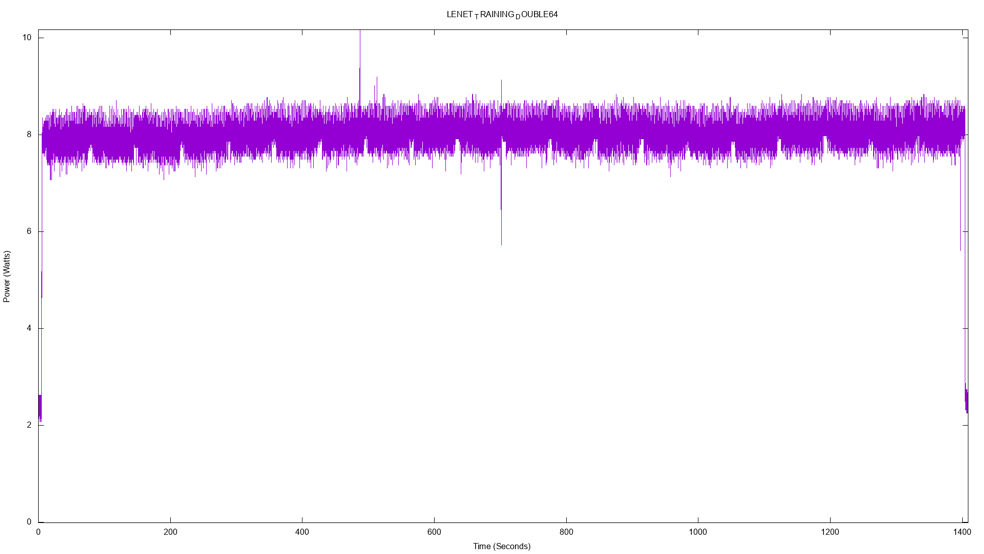
\includegraphics[width=85mm,scale=1]{lenet_train_double.png}
              \caption{Training LeNet on MNIST dataset, in double precision}
              \label{lenet_train_double}
          \end{figure}

          \begin{figure}[h]
              \centering
              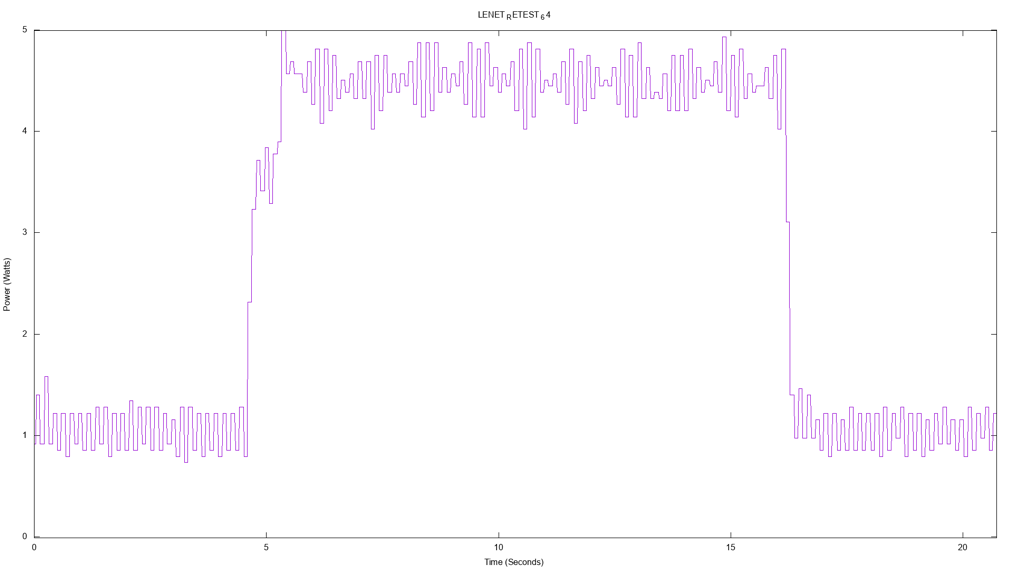
\includegraphics[width=85mm,scale=1]{lenet_test_double.png}
              \caption{Testing LeNet on MNIST dataset, in double precision}
              \label{lenet_test_double}
          \end{figure}

          \begin{figure}[h]
              \centering
              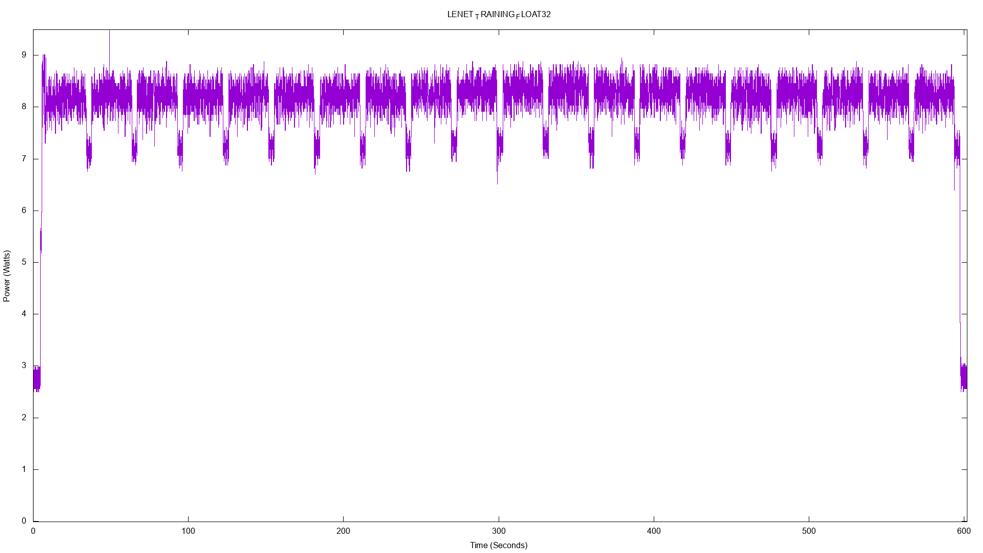
\includegraphics[width=85mm,scale=1]{lenet_train_single.png}
              \caption{Testing LeNet on MNIST dataset, in single precision}
              \label{lenet_train_single}
          \end{figure}
          
          \begin{figure}[h]
              \centering
              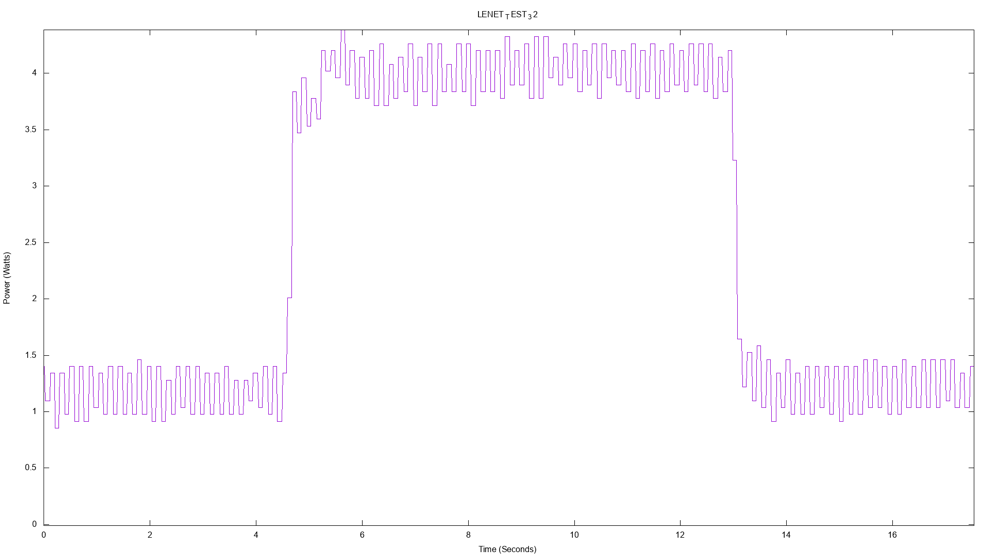
\includegraphics[width=85mm,scale=1]{lenet_test_single.png}
              \caption{Testing LeNet on MNIST dataset, in single precision}
              \label{lenet_test_single}
          \end{figure}
          
          \begin{figure}[h]
              \centering
              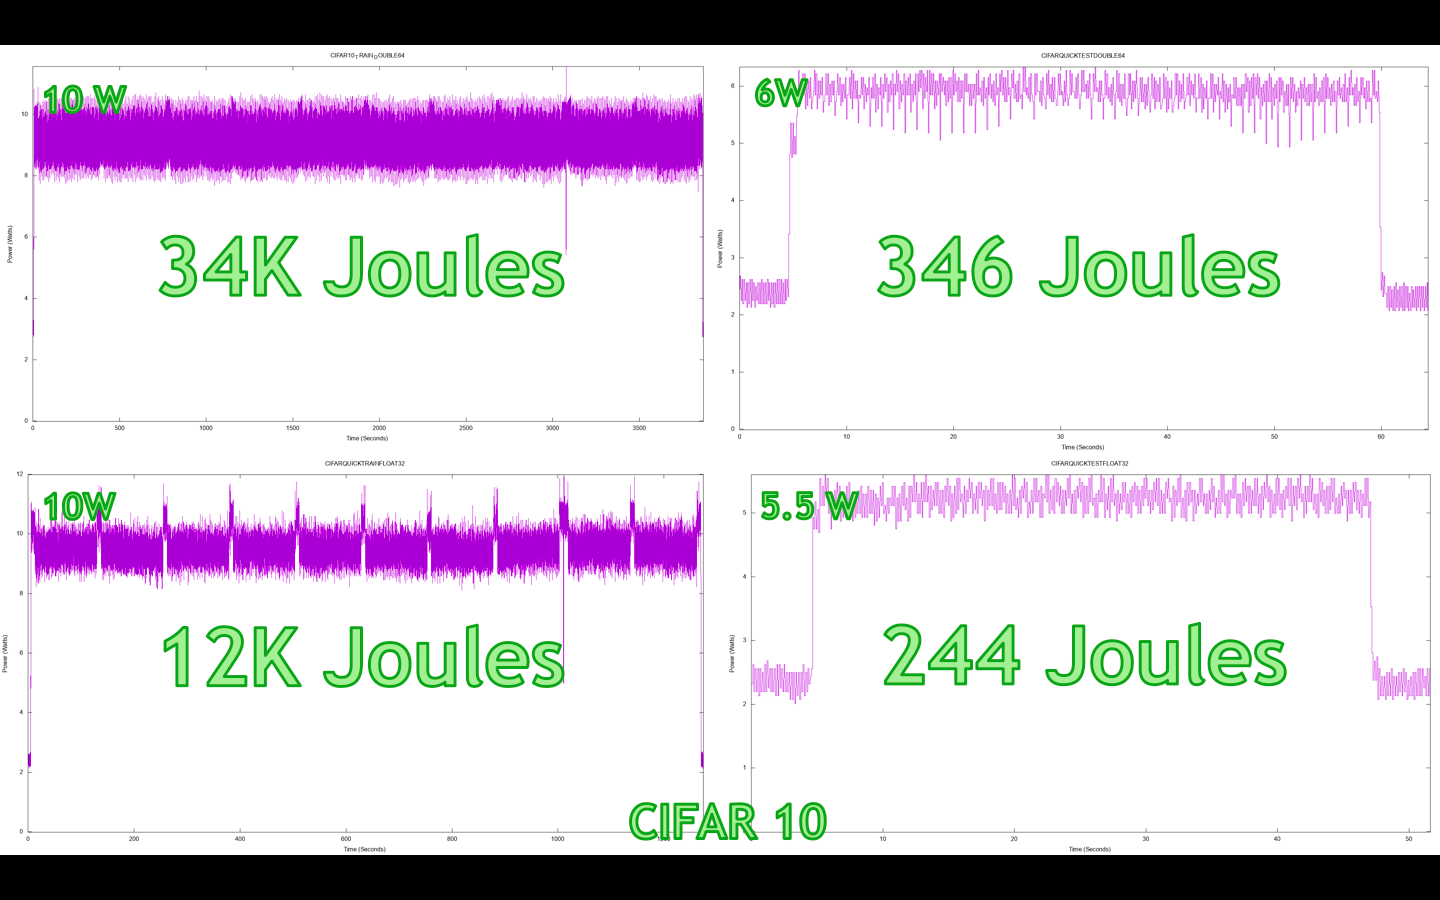
\includegraphics[width=85mm,scale=1]{cifar10.png}
              \caption{A sample Madonna Pass, analyzing Cuda-Convnet on CIFAR-10 dataset}
              \label{cifar}
          \end{figure}
          
          \begin{figure}[h]
              \centering
              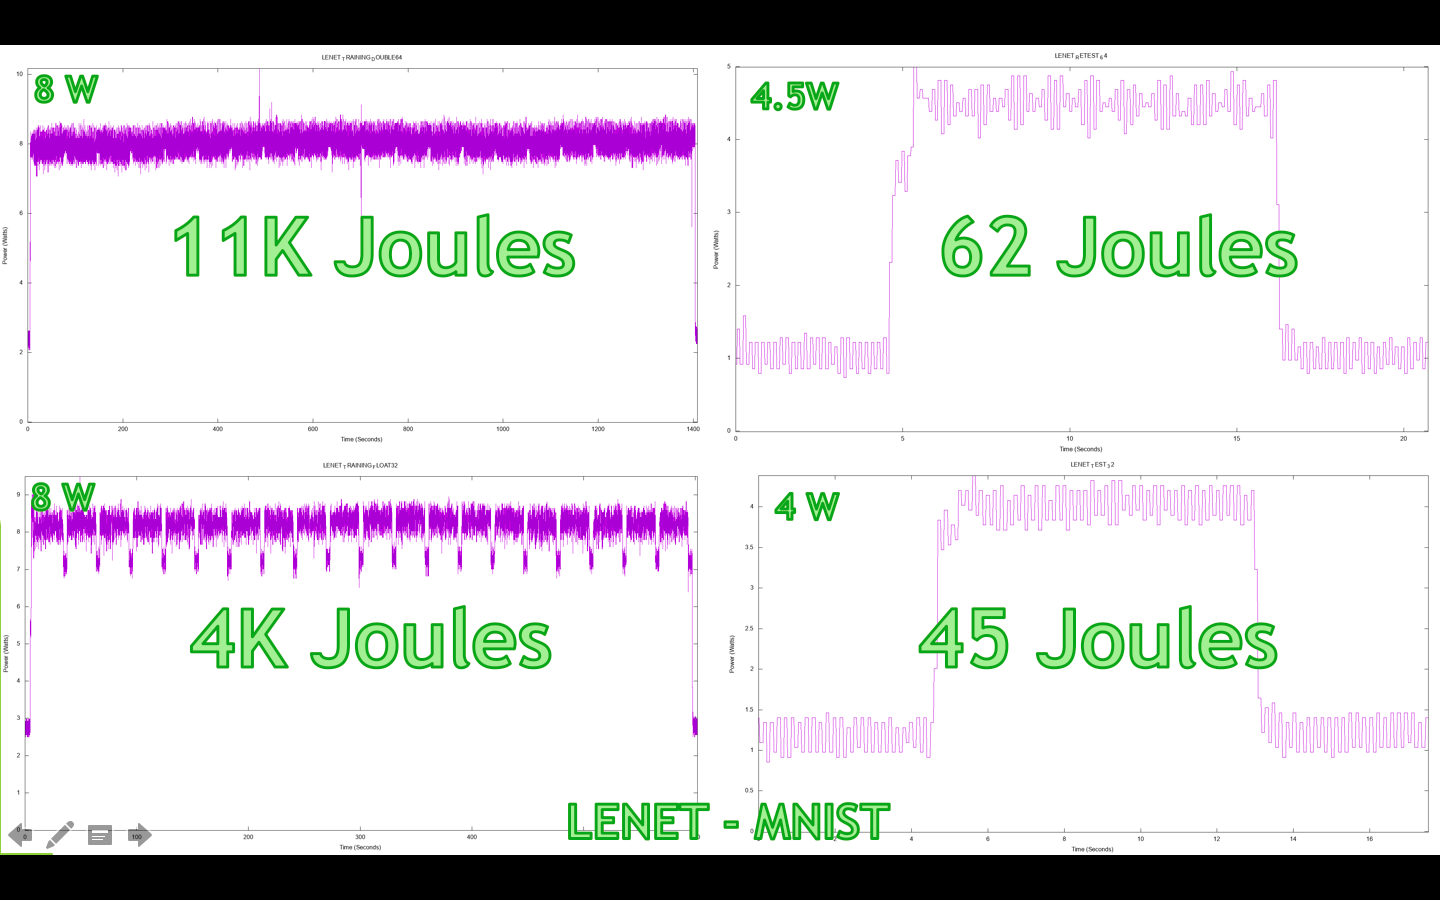
\includegraphics[width=85mm,scale=1]{lenet.png}
              \caption{A sample Madonna Pass, analyzing LeNet on MNIST dataset}
              \label{lenet}
          \end{figure}


\section{DISCUSSION}

\subsection{Assistance in MADONNA}
\subsection{Lessons Learnied using developing MADONNA v1.0}

\section{RELATED WORK}

\subsection{Minerva}

\section{CONCLUSIONS}

A conclusion section is not required. Although a conclusion may review the main points of the paper, do not replicate the abstract as the conclusion. A conclusion might elaborate on the importance of the work or suggest applications and extensions. 

\begin{thebibliography}{99}

\bibitem{c1} Minerva: Enabling Low-Power, Highly-Accurate
Deep Neural Network Accelerators
Brandon Reagen Paul Whatmough Robert Adolf Saketh Rama
Hyunkwang Lee Sae Kyu Lee José Miguel Hernández-Lobato
Gu-Yeon Wei David Brooks
Harvard University, 2016 

\end{thebibliography}

\end{document}
